\documentclass[tikz]{standalone}

\usepackage[T1]{fontenc}
\usepackage[english]{babel}

\usetikzlibrary{3d, calc}

\usepackage{amsmath}

\usepackage{standalone}

\begin{document}
	\begin{tikzpicture}
		\node (image) {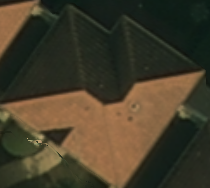
\includegraphics[width=3cm]{images/features/image/elancourt-39322}};

		\path (image.north east) + (0, 1) node[anchor=south east] (model) {\includestandalone[mode=buildnew, width=3cm]{figures/building_model}};

		\path (image.east) + (2.7, .2) node[anchor=west] (blue_channel) {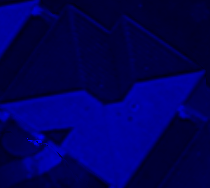
\includegraphics[width=3cm]{images/features/image/elancourt-39322_b}};
		\path (blue_channel) + (-.2, -.2) node (green_channel) {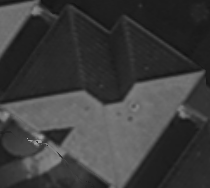
\includegraphics[width=3cm]{images/features/image/elancourt-39322_g}};
		\path (green_channel) + (-.2, -.2) node (red_channel) {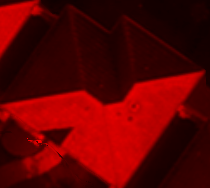
\includegraphics[width=3cm]{images/features/image/elancourt-39322_r}};
		\draw[->, very thick] (image.east) -- (red_channel.west |- green_channel);
		

		\path (green_channel |- model) node (mask) {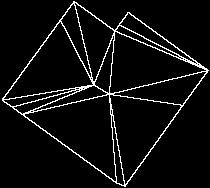
\includegraphics[width=3cm]{images/features/image/elancourt-39322_mask}};
		\draw[->, very thick] (model.east) -- (mask.west);

		\path (mask.north) node[anchor=south, text width=3cm] (mask_legend) {\footnotesize \subcaption{Nadir Projection. \label{subfig::nadir_c}}};
        \path (model |- mask_legend.north) node[anchor=north, text width=3cm] (model_legend) {\footnotesize \subcaption{\gls{acr::3d} model. \label{subfig::input_c}}};

		\path (green_channel.east) + (3, 0) node[anchor=west] (green_mask_channel) {};
		\path (green_mask_channel) + (.3, .3) node (mask_channel) {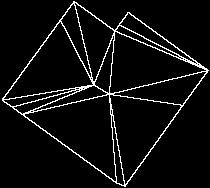
\includegraphics[width=3cm]{images/features/image/elancourt-39322_mask}};
		\path (green_mask_channel) + (.1, .1) node (blue_channel_channel) {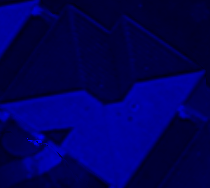
\includegraphics[width=3cm]{images/features/image/elancourt-39322_b}};
		\path (green_mask_channel) + (-.1, -.1) node (green_channel_channel) {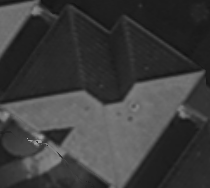
\includegraphics[width=3cm]{images/features/image/elancourt-39322_g}};
		\path (green_mask_channel) + (-.3, -.3) node (red_channel_channel) {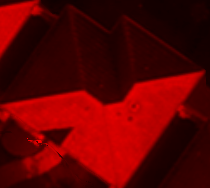
\includegraphics[width=3cm]{images/features/image/elancourt-39322_r}};
        \path (green_mask_channel.south |- red_channel_channel.south) node[anchor=north, text width=3cm] (channel_legend) {\footnotesize \subcaption{Late fusion: \texttt{channel}. \label{subfig::early}}};

        \path (green_channel |- channel_legend.north) node[anchor=north, text width=3cm] (rgb_legend) {\footnotesize \subcaption{RGB channels. \label{subfig::rgb_c}}};
        \path (image |- channel_legend.north) node[anchor=north, text width=3cm] (image_legend) {\footnotesize \subcaption{Orthoimage. \label{subfig::orthoimage_c}}};

		\draw[->, very thick] (green_channel.east) -- (red_channel_channel.west |- green_mask_channel);
		\draw[very thick] (mask.east) -- ($(mask)!.5!(green_mask_channel |- mask)$) -- ($(green_channel)!.5!(green_mask_channel)$);
	\end{tikzpicture}
\end{document}
